\chapter{Pendahuluan}
\label{chap:pendahuluan}

Bab ini membahas tentang latar belakang, rumusan masalah, tujuan, batasan masalah, metodologi penelitian, dan sistematika pembahasan dari skripsi ini.

\section{Latar Belakang}
\label{sec:label}
Calcudoku, atau dikenal juga sebagai KenKen, atau Mathdoku, adalah sebuah permainan teka-teki (\textit{puzzle}) angka yang untuk menyelesaikannya memerlukan perpaduan dari logika dan kemampuan aritmatika yang sederhana. Permainan ini adalah sebuah permainan teka-teki logika yang sederhana, namun, untuk menemukan solusinya cukup rumit, terutama untuk masalah yang lebih susah.

Teka-teki ini mirip dengan Sudoku. Sudoku adalah sebuah permainan teka-teki angka dengan \textit{grid} berukuran \begin{math}n^2\end{math}, di mana dalam setiap baris, kolom, dan \begin{math}n^2\end{math} area yang berukuran \begin{math}n \times n\end{math} tidak boleh ada angka yang berulang, dengan \begin{math}n\end{math} adalah ukuran area. Biasanya, \begin{math}n = 3\end{math}, sehingga \textit{grid} berukuran \begin{math}9 \times 9\end{math}, dan ada 9 area yang berukuran \begin{math}3 \times 3\end{math}. Contoh permainan teka-teki Sudoku dapat dilihat pada Gambar~\ref{fig:sudoku}.

\begin{figure}
\centering
\captionsetup{justification=centering}
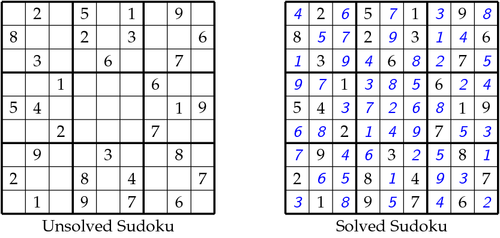
\includegraphics[scale=0.5]{Pendahuluan/Sudoku.png}
\caption[Contoh permainan teka-teki Sudoku dengan solusinya]{Contoh permainan teka-teki Sudoku dengan solusinya}
\label{fig:sudoku}
\end{figure}

Persamaannya, tujuan dari teka-teki ini adalah mengisi setiap sel (\textit{cell}) dalam (\textit{grid}) dengan angka 1 sampai \begin{math}n\end{math} tanpa pengulangan angka dalam setiap kolomnya dan barisnya untuk \textit{grid} berukuran \begin{math}n \times n\end{math}, dengan \begin{math}n\end{math} adalah ukuran \textit{grid}. Tidak ada angka yang boleh muncul lebih dari sekali dalam setiap baris atau kolom dalam \textit{grid}.

Perbedaannya, jika pada Sudoku \textit{grid} berukuran \begin{math}n \times n\end{math} dibagi menjadi \begin{math}n\end{math} (\textit{cage}) dengan setiap \textit{cage} terdiri atas \begin{math}n\end{math} sel, pada Calcudoku \textit{grid} dibagi menjadi sejumlah \textit{cage} yang jumlah selnya bervariasi. Setiap \textit{cage} dibatasi oleh garis yang lebih tebal daripada garis pembatas antar sel. Angka-angka dalam satu \textit{cage} yang sama harus menghasilkan angka tujuan yang telah ditentukan jika dihitung menggunakan operasi matematika yang telah ditentukan (penjumlahan, pengurangan, perkalian, atau pembagian). Angka-angka dalam satu \textit{cage} juga boleh berulang, selama pengulangan tidak terjadi dalam satu kolom atau baris yang sama. Jika \textit{cage} hanya berisi satu sel, maka satu-satunya kemungkinan jawaban untuk sel tersebut adalah angka tujuan dari \textit{cage} tersebut. Angka tujuan dan operasi matematika dituliskan di sudut kiri atas \textit{cage}. Pada awalnya, setiap sel dalam setiap \textit{cage} dalam teka-teki ini kosong, belum terisi oleh angka-angka. \textit{Border line} adalah garis pembatas terluar, \textit{row line} adalah garis pembatas antar baris, dan \textit{column line} adalah garis pembatas antar kolom. Gambar~\ref{fig:hybrid1} menggambarkan contoh sebuah permainan teka-teki Calcudoku ~\cite{fahda:16:backtracking} ~\cite{johanna:12:hybrid}.

\begin{figure}
\centering
\captionsetup{justification=centering}
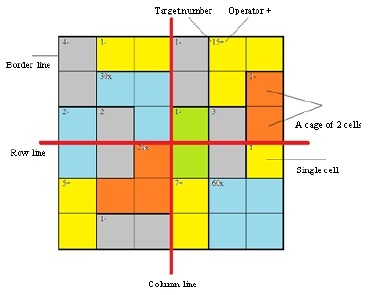
\includegraphics[scale=0.5]{Gambar/HybridGenetic1}
\caption[Contoh permainan teka-teki Calcudoku dengan penjelasan tentang elemen-elemen dari teka-teki ini ~\cite{johanna:12:hybrid}]{Contoh permainan teka-teki Calcudoku dengan penjelasan elemen-elemen dari teka-teki ini ~\cite{johanna:12:hybrid}}
\label{fig:hybrid1}
\end{figure}

Calcudoku dapat diselesaikan menggunakan beberapa algoritma. Skripsi ini membahas tentang penyelesaian Calcudoku menggunakan algoritma \textit{backtracking} dan algoritma \textit{hybrid genetic}, dan perbandingan performansi \textit{performance} antara kedua algoritma tersebut dalam hal kecepatan dan kesuksesan dalam menyelesaikan Calcudoku.

Algoritma \textit{backtracking} adalah sebuah algoritma umum yang mencari solusi dengan mencoba salah satu dari beberapa pilihan, jika pilihan yang dipilih ternyata salah, komputasi dimulai lagi pada titik pilihan dan mencoba pilihan lainnya. Untuk bisa melacak kembali langkah-langkah yang telah dipilih, maka algoritma harus secara eksplisit menyimpan jejak dari setiap langkah yang sudah pernah dipilih, atau menggunakan rekursi (\textit{recursion}). Rekursi dipilih karena jauh lebih mudah daripada harus menyimpan jejak setiap langkah yang pernah dipilih, hal ini menyebabkan algoritma ini biasanya berbasis DFS (\textit{Depth First Search}) ~\cite{fahda:16:backtracking}.

Algoritma \textit{rule based} adalah sebuah algoritma berbasis aturan logika untuk menyelesaikan permainan teka-teki Sudoku dan variasinya, termasuk Calcudoku. Beberapa aturan logika yang digunakan dalam algoritma ini adalah \textit{single square rule}, \textit{naked subset rule}, \textit{hidden single rule}, \textit{evil twin rule}, \textit{killer combination}, dan \textit{X-wing}.

Pencarian heuristik adalah sebuah teknik pencarian kecerdasan buatan (\textit{artifical intelligence}) yang menggunakan heuristik dalam langkah-langkahnya. Heuristik adalah semacam aturan tidak tertulis yang mungkin menghasilkan solusi. Heuristik kadang-kadang efektif, tetapi tidak dijamin akan berhasil. dalam setiap kasus. Heuristik memerankan peran penting dalam strategi pencarian karena sifat eksponensial dari kebanyakan masalah. Heuristik membantu mengurangi jumlah alternatif solusi dari angka yang bersifat eksponensial menjadi angka yang bersifat polinomial. Contoh teknik pencarian heuristik adalah \textit{Generate and Test}, \textit{Hill Climbing}, dan \textit{Best First Search}.

Algoritma genetik adalah salah satu teknik heuristik \textit{Generate and Test} yang terinspirasi oleh sistem seleksi alam. Algoritma ini adalah perpaduan dari bidang biologi dan ilmu komputer. Algoritma ini adalah salah satu dari teknik pencarian heuristik.

Algoritma ini memanipulasi informasi, biasanya disebut sebagai kromosom. Kromosom ini mengkodekan kemungkinan jawaban untuk sebuah masalah yang diberikan. Kromosom dievaluasi dan diberi \textit{fitness value} berdasarkan seberapa baikkah kromosom dalam menyelesaikan maslah yang diberikan berdasarkan kriteria yang ditentukan oleh pembuat program. Nilai kelayakan ini digunakan sebagai probabilitas kebertahanan hidup kromosom dalam satu siklus reproduksi. Kromosom baru (kromosom anak, \textit{child chromosome}) diproduksi dengan menggabungkan dua (atau lebih) kromosom orang tua (\textit{parent chromosome}). Proses ini dirancang untuk menghasilkan kromosom-kromosom keturunan yang lebih layak, kromosom-kromosom ini menyandikan jawaban yang lebih baik, sampai solusi yang baik dan yang bisa diterima ditemukan.

Algoritma \textit{hybrid genetic} adalah gabungan antara algoritma genetik dan algoritma-algoritma lainnya. Dalam kasus ini, algoritma genetik digabungkan dengan algoritma \textit{rule based}. Algoritma \textit{rule based} akan dijalankan sampai pada titik dimana algoritma tidak bisa menyelesaikan permainan teka-teki Calcudoku. Jika algoritma sudah tidak bisa menyelesaikan permainan, maka algoritma genetik akan mulai dijalankan ~\cite{johanna:12:hybrid}.

\section{Rumusan Masalah}
\label{sec:rumusan}
Berdasarkan latar belakang yang telah diuraikan di atas, dapat dirumuskan permasalahan sebagai berikut:
\begin{enumerate}
\item Bagaimana cara mengimplementasikan perangkat lunak (\textit{software}) permainan teka-teki Calcudoku?
\item Bagaimana cara mengimplementasikan algoritma \textit{backtracking} untuk menyelesaikan Calcudoku?
\item Bagaimana cara mengimplementasikan algoritma \textit{hybrid genetic} untuk menyelesaikan Calcudoku?
\item Bagaimana perbandingan performansi algoritma \textit{backtracking} dengan algoritma \textit{hybrid genetic} dalam menyelesaikan Calcudoku?
\end{enumerate}

\section{Tujuan}
\label{sec:tujuan}
Berdasarkan rumusan masalah yang telah dirumuskan, maka tujuan dari pembuatan skripsi ini adalah:
\begin{enumerate}
\item Membuat perangkat lunak solusi permainan teka-teki Calcudoku yang menerima input berupa soal teka-teki dan mampu menyelesaikan soal teka-teki tersebut menggunakan algoritma \textit{backtracking} dan \textit{hybrid genetic}.
\item Membandingkan performansi algoritma \textit{backtracking} dengan algoritma \textit{hybrid genetic} dalam hal kesuksesan dan (jika sukses) kecepatan dalam menyelesaikan Calcudoku.
\end{enumerate}

\clearpage

\section{Batasan Masalah}
\label{sec:batasan}
Ruang lingkup dari skripsi ini dibatasi oleh batasan-batasan masalah sebagai berikut:
\begin{enumerate}
\item Ukuran \textit{grid} untuk permainan teka-teki Calcudoku adalah antara \begin{math}4 \times 4\end{math} sampai dengan \begin{math}8 \times 8\end{math}. Pada awalnya, ukuran \textit{grid} direncanakan akan dibatasi dari \begin{math}3 \times 3\end{math} sampai dengan \begin{math}9 \times 9\end{math}, tetapi karena kurangnya contoh soal teka-teki Calcudoku dengan ukuran \begin{math}3 \times 3\end{math}, dan ada masalah saat pengujian (keluar pesan error "\textit{Memory full}" saat menguji \textit{solver} dengan algoritma \textit{backtracking} pada \textit{grid} yang berukuran \begin{math}9 \times 9\end{math}, maka ukuran \textit{grid} dibatasi dari \begin{math}4 \times 4\end{math} sampai dengan \begin{math}8 \times 8\end{math}.
\item Pada algoritma \textit{rule based}, yang merupakan bagian dari algoritma \textit{hybrid genetic}, aturan-aturan logika yang digunakan dibatasi hanya pada aturan \textit{single square}, \textit{naked single}, \textit{naked double}, \textit{hidden single}, dan \textit{killer combination}.
\item Soal-soal permainan teka-teki Calcudoku yang digunakan dalam pengujian diambil dari sumber-sumber berikut:
	\begin{enumerate}
	\item \url{https://iota.math.msu.edu/k12-outreach/kenken-puzzles/}
	\item \url{http://thinkmath.edc.org/resource/kenken-puzzles}
	\end{enumerate}
\end{enumerate}

\section{Metodologi Penelitian}
\label{sec:metlit}
Langkah-langkah yang akan dilakukan dalam pembuatan skripsi ini adalah:
\begin{enumerate}
\item Studi literatur
	\begin{enumerate}
	\item Melakukan studi literatur tentang permainan teka-teki Calcudoku.
	\item Melakukan studi literatur tentang algoritma \textit{backtracking}.
	\item Melakukan studi literatur tentang algoritma \textit{rule based} dan algoritma genetik.
	\end{enumerate}
\item Analisis, perancangan, dan pengembangan perangkat lunak
	\begin{enumerate}
	\item Melakukan analisis dan menentukan fitur-fitur yang diperlukan dalam perangkat lunak permainan teka-teki Calcudoku.
	\item Membuat perangkat lunak Calcudoku dengan fitur-fitur yang telah ditentukan. 
	\item Mengimplementasikan algoritma \textit{backtracking} untuk Calcudoku.
	\item Mengimplementasikan algoritma \textit{hybrid genetic} untuk Calcudoku.
	\end{enumerate}
\item Melakukan pengujian dan eksperimen terhadap perangkat lunak Calcudoku yang telah dibuat. Soal-soal permainan teka-teki Calcudoku yang digunakan dalam pengujian diambil dari sumber-sumber berikut:
	\begin{enumerate}
	\item \url{https://iota.math.msu.edu/k12-outreach/kenken-puzzles/}
	\item \url{http://thinkmath.edc.org/resource/kenken-puzzles}
	\end{enumerate}
\item Membandingkan performansi algoritma \textit{backtracking} dengan algoritma \textit{hybrid genetic} dalam menyelesaikan Calcudoku.
\item Membuat kesimpulan berdasarkan hasil pengujian perangkat lunak yang telah dibuat.
\end{enumerate}

\section{Sistematika Pembahasan}
\label{sec:sispem}
Sistematika pembahasan skripsi ini adalah sebagai berikut:
\begin{enumerate}
\item Bab 1 berisi latar belakang, rumusan masalah, tujuan, batasan masalah, metodologi penelitian, dan sistematika pembahasan dari skripsi ini.
\item Bab 2 membahas tentang landasan teori yang digunakan dalam skripsi ini, yaitu tentang permainan teka-teki Calcudoku, algoritma \textit{backtracking} dan algoritma \textit{hybrid genetic}.
\item Bab 3 membahas tentang analisis perangkat lunak Calcudoku dan analisis algoritma \textit{backtracking} dan algoritma \textit{hybrid genetic}.
\item Bab 4 membahas tentang perancangan dan pembuatan perangkat lunak Calcudoku dan algoritma \textit{backtracking} dan algoritma \textit{hybrid genetic} untuk menyelesaikan permainan, perancangan antarmuka (\textit{interface}), input dan output, diagram kelas (\textit{class diagram}), dan diagram aktivitas (\textit{activity diagram}).
\item Bab 5 membahas tentang implementasi dari perangkat lunak Calcudoku dan algoritma \textit{backtracking} dan algoritma \textit{hybrid genetic} yang telah dirancang, implementasi antarmuka, input dan output yang telah dirancang, dan pengujian perangkat lunak Calcudoku dalam hal perbandingan performansi algoritma \textit{backtracking} dan algoritma \textit{hybrid genetic} dalam menyelesaikan permainan.
\item Bab 6 berisi simpulan dari pembuatan perangkat lunak Calcudoku dan hasil pengujiannya, dan saran untuk penelitian pengembangan perangkat lunak selanjutnya.
\end{enumerate}